% -*- mode: latex; eval: (flyspell-mode 1) -*-
\documentclass[fontsize=12,a4paper]{scrartcl}


\usepackage[T1]{fontenc}

\usepackage[narrow]{inconsolata}
\usepackage{gentium}

\usepackage{gensymb}
%\usepackage{minted}
\usepackage{hyperref}
\usepackage{graphicx}
\usepackage{xcolor}
\usepackage{framed}
%\usepackage{makeidx}
\usepackage{amsmath}
\usepackage{hyperref}
\usepackage{natbib}
\usepackage[utf8]{inputenc}
\usepackage{rotating}

% \usepackage{tocloft}
% \setlength{\cftsecnumwidth}{2.5em}
% \setlength{\cftsubsecnumwidth}{3.5em}

\DeclareMathOperator{\round}{round}

\makeindex

\newenvironment{warning}{\begin{framed}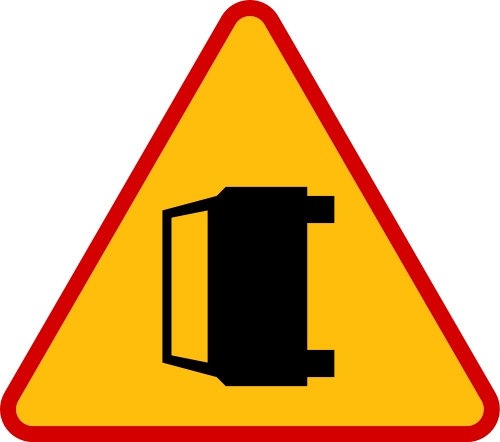
\includegraphics[width=5em]{accident-area-ahead.png}
}{\end{framed}}


\pagestyle{headings}

\bibliographystyle{alpha}

\begin{document}

\title{Concurrency Architecture of the MOONS fpu\_driver Module}


\author{Johannes Nix}

\maketitle

\tableofcontents

\section{Related documents}

\begin{tabular}{|ll|}
  \hline
\verb+[1] VLT-TRE-MON-14620-1018+, &  FPU Verification Requirements \\
\verb+[2] VLT-TRE-MON-14620-3017+, & MOONS Fibre Positioner Verification Software Design \\
\verb+[3] VLT-TRE-MON-14620-3016+, & Fibre Positioner Communication Protocol\\
\verb+[4] FPUMovementSafetySpecification+ & Specification of safety levels for FPU movements\\
\verb+[5] VLT-ICD-MON-14620-4303+ & RFE to Instrument Software Interface Control Document \\
\hline
\end{tabular}


\section{Scope of this document}

The goal of this document is to explain the main points of the
concurrency architecture of the \texttt{fpu\_driver}.  This is
necessary because, unlike many other aspects, in C/C++ source code,
the concurrency behaviour is not explicitly defined.  One would need
to scrutinize the entire source code to understand it.

At the same time, failure to ensure synchronized access
in concurrent code can be the cause for hard-to-debug
undefined behaviour \cite{Regehr:AGtUBPt3}\cite{MeyersAlexandrescu:2004:DCL}.

\section{Overview}

\subsection{Basic operation: Gateways, sockets and queues}

At the most fundamental level, the driver module generates CAN
messages which are sent to three different gateways, via several
socket connections. The gateways forward the messages to FPUs via 15
CAN buses, and the FPUs usually send responses. The responses are
received by the driver, which tracks the state of each FPU.

The driver tries to send messages as fast as possible. Because the
bandwidth of the socket connection and, more importantly, the CAN
buses, is limited, the driver does this in such a way so that it does
not lose waiting time: If it cannot write to one socket, it looks
whether there is a message which can be sent to another socket, and if
this is the case, it proceeds with this message.

To do that, messages are stored in three queues, one for each
gateway.That means that when sending messages, it has to match sockets
which can transmit new messages with queues that have messages that
should be delivered.

The basic architecture is somewhat shaped like modern server
architectures which solve the so-called C10k problem, that is, being
able to maintain tens of thousands of connections in a single server
process\cite{Kegel:C10kProblem}\cite{WP:C10kProblem}.

In traditional server architectures, which use one thread for every
connection, this is not possible, because the cost for switching
between threads is high, if many threads are involved. Applied to the
task of communicating with 1000 FPUs, it is not efficient to have one
thread for every FPU. Rather, there is exactly one thread which sends
messages, and one thread which receives them, and the method for
sending and receiving data are so-called non-blocking function calls.
This reduces the amount of locking and synchronization needed.

\subsection{Concurrency architecture}
\begin{sidewaysfigure}[p]
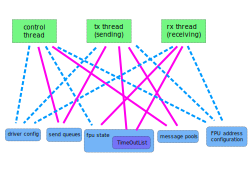
\includegraphics[width=0.9\textwidth]{fpu-driver-concurrency-architecture.png}
\caption[Overview of Concurrency architecture of FPU driver]{Overview
  of Concurrency architecture of FPU driver. The green rectangles are
  threads, the blue rounded rectangles are shared data structures, and
  the arrows show how the threads access the data structures: broken
  blue arrows denote read-only access, and solid magenta arrows
  indicate modifying, or read-write access.}
\label{fig:overview}
\end{sidewaysfigure}

\subsection{Sockets}


Sockets are identified by socket file descriptors.  Using these socket
file descriptors is thread-safe, as long as not different threads try
to simultaneously write to, or read from, the same socket. The driver
architecture guarantees that this does not happen: Writing to the
sockets happens always in the tx thread, and reading from the sockets
happens always in the rx thread.  These operations are
thread-safe. Because sockets are normally not opened or closed during
the existence of the threads, their state does not need to be checked
apart from the check of return codes of the \texttt{send()} and
\texttt{recv()} operations. If a socket connection fails, the error is
detected by checking the return codes of \texttt{send()} and
\texttt{recv()}, the sending (tx) and receiving (rx) loops are exited,
and the threads are terminated.


\subsection{Threads}
Figure~\ref{fig:overview} gives an overview on the concurrency
structure in the \texttt{fpu\_driver} module.


In the top row of the figure we see three rectangles,
which represent the three threads which are active
in the running \texttt{fpu\_driver} module. These are:

\begin{description}
\item[Control thread] The ``control''  thread is identical to the main thread of
  the program. It's functions are entered when new commands are sent
  to the FPUs, and return when the result of the commands is returned
  to the caller. In the time between, the thread could be
  blocked. This works almost exactly as in the same way
  as, for example, a \texttt{read()} or \texttt{write()} library
  call in a program that uses POSIX file IO.


\item[tx thread] The ``tx'' thread performs the sending of commands to
  the fibre positioners, by sending messages over three socket
  connections. Each socket is connected to one EtherCAN gateway. It is
  structured so that it can send messages as fast as possible. If the
  gateways or the FPUs cannot process messages as fast, it waits until
  one of the sockets is writable. The sockets are shared between tx
  thread and rx thread.

\item[rx thread] The ``rx'' thread reads any return messages from the
  fibre positioners to the driver, and updates the driver's internal
  structures which describe the state of the FPUs. It is designed so
  that it can read messages as fast as possible. Especially, the rx
  thread is designed so that it never has to wait itself for any
  long-running or potentially blocking operation, such as a file read,
  or a network response\footnote{There is one exception to this, which
    is logging of detailed debug messages if a high level of verbosity
    is selected. In this case, there are blocking calls to the log
    functions, which could block the rx thread temporarily. Such a
    high level will slow down operation and is not advisable for
    normal operation.}.

\end{description}


\subsection{Data structures}

The rounded boxes in the bottom of the figure represent the main data
structures which these three threads are accessing.

The arrows show the type of access. There are two types of access,
read-only access, which is symbolized by broken blue arrows, and
modifying access, which is depicted by magenta straight arrows. We see
that there are two data structures which are different, in that they
only receive read-only access from all three threads. As matters
around them are simpler, we will discuss them first.

\subsubsection{Read-only data}

The read-only data structures are as follows:

\begin{description}
\item[Driver configuration] This structure holds the parameters which
  define the global configuration of the driver, for example the
  minimum motor frequency required in waveforms. It has the type
  \texttt{EtherCANInterfaceConfig}, and is passed as a constant
  argument to the driver's constructor. Because it is in no place
  modified, we know that it does not change, and we can pass it
  everywhere as constant (similar as a string in Python).

  (In the core FPU driver, these parameters are passed as a constant
  structure. Passing the configuration in memory has the advantage
  that the core driver does not become dependent on the ESO VLT
  framework, and this makes it possible to test it within the FPU
  verification system, which cannot depend on that framework.)

\item[FPU address configuration] This structure is a table which maps
  the logical FPU numbers to the address triplet of (gateway number,
  bus number, and CAN ID on the bus). The table is created at program
  start-up, and passed to the threads when they are created\footnote{
    As is the case with the driver parameters, the address
    configuration is determined at start-up time. Currently, the
    address table is passed to the method
    \texttt{GatewayInterface::connect()}. The final driver version
    will read the addresses from a configuration file and, for
    example, pass it to the \texttt{connect()} method.}.

  Synchronization of the table poses an interesting question: If the
  table is created at program start-up, it is modified in the control
  thread. After this, the tx thread and the rx thread are created. How
  can we be sure that this modification is not seen in the newly
  created threads?

  The answer to this is that the creation of threads in pthreads
  causes a so-called memory barrier
  \cite{WP:MemoryBarrier}\cite{Preshing:2012:MemoryBarriers}.  Any
  data which was written by the CPU before that thread was created, is
  written to memory before the new thread can see it. This is
  important, because normally in a C program with different threads,
  there is \emph{no} notion of ``before'' or ``after'' for operations
  in different threads, unless such operations are explicitly
  synchronized. The thread creation represents such an synchronization
  point.



\end{description}

\subsection{Message queues}
Furthermore, we have three main types of data structures which are not
only read concurrently, but also modified. We discuss the message
queues first.

Message queues are thread-safe data structures which allow the control
thread to send parametric messages for individual FPUs to the tx
thread. The control thread is responsible for setting up the messages
and its actual data content, and the tx thread is responsible for
sending them to a gateway.

To achieve that, the control thread inserts each message into a data
structure which is basically a thread-safe FIFO or ring buffer.  The
insertion method uses locks to ensure that the internal invariants of
the data structure are kept correct, and that no unsynchronized
concurrent modifications occur. There is one message queue for each
socket, so that we have three of them. Using the FPU's address
configuration, the control thread knows into which queue to insert a
message.

The tx thread checks whether there are messages in the message queues,
\emph{and} whether it can send a message to a socket without blocking
(this is done using the \texttt{ppoll()} syscall). If this is the
case, the message is serialized into a byte sequence and written to
the socket; the remaining processing is handled by the OS kernel.



\subsection{Message pools}

One aspect which needs to be discussed now is what happens with the
message after it was processed by the rx thread. This is related to
how messages are represented as objects in memory. Messages could be
just values which are copied, and handled by a few functions. However,
it is actually useful to treat them as object instances which have
virtual methods, supporting some degree of abstraction by using
object-oriented programming techniques.

As such objects can have different sizes, they need to be passed by
pointers, and their memory needs to be managed.  This is done by C++
smart pointers (more precisely, \texttt{std::shared\_ptr<>}, which are
supported by C++11 and newer versions of C++). In theory, each message
object could be allocated, using \texttt{new}, when it is needed, and
deallocated, using \texttt{delete}, when it is not longer
needed. However this is relatively slow. Therefore, when messages
instances are needed, these are taken from a set of message pools,
which are created on program start-up, and these instances are
inserted back into the corresponding pool when they are not needed any
more at the moment.

The resulting pattern is that the control thread takes a message
instance from a message pool, and inserts a reference to it into a
message queue. Then, the tx thread pops it from the message queue,
generates and sends its byte representation to the socket it is
addressed to, and recycles the message memory by adding its reference
again to the corresponding message pool. With this scheme, no dynamic
allocation of messages is needed after program start-up, so this is
much faster.

As a detail, there is one pool for each type of message, and the pools
are simpler organized than the message queues, they are basically a
stack of smart pointers, implemented as a \texttt{std::vector<std::shared\_ptr<\ldots>>>}.

\subsection{FPU state handling}

After looking at the message queues and message queues, we can now
look at the remaining data structure, which is more complex, and very
central to the FPU driver software. It is represented by the larger
rectangular box in the middle of figure~\ref{fig:overview}, and
provides an array of structs which record the FPU's state with each
response message that was received from the gateway. Because we have
one such state record for each of the 1001 FPUs, this structure is
called the \texttt{FPU\_state} array, or \texttt{FPUArray}.

For the moment, we will temporarily ignore the box which is labelled
``\texttt{TimeOutList}'', which will be explained soon.  The responses
messages are received by the rx thread, of course.  Upon receipt, the
rx thread writes the state updates into the FPU state array,
symbolized by the magenta arrow. The control thread reads from the
state array. To avoid corruption by concurrent modification, it uses a
lock or Mutex, which ensures that write accesses and read accesses are
mutually exclusive. The rx thread keeps this lock most of the
time. Only for short moments, the lock gets released, which gives the
control thread the opportunity to read back the new state data, and
return it to the caller of the driver method.

\paragraph{Transfer of state data from rx to control thread}
As the reader might already guess, the FPU state structure is updated
by the rx thread, but it is also passed to the control thread, and its
information is required by the higher levels of application software
which use the driver methods. In theory, this data could be protected
by holding more locks. But this would violate the requirement that we
want the rx thread to accept and store that data as fast as possible.

Instead, the FPU state data is \emph{copied} when it is passed from
the rx thread to the control thread. Only while that copy is
performed, it needs to be locked for the rx thread. And because the
copy is a fast memory operation with nothing that can block, the time
the lock needs to be hold is very short. As a result, the control
thread methods return a copy of the FPU state data, which can be
processed conveniently without any locking.

\subsection{The \texttt{TimeOutList} data structure}

Noe, let's have a look at the data structure \texttt{TimeOutList},
which is written to by both the tx thread, and the rx thread. Its
function is as follows:

Normally, most messages to an FPU are promptly followed by a response
within a few milliseconds. However, it can happen that this runs into
errors, for example if the connection to the CAN bus gets broken. In
this case, the response will never arrive, and the driver needs to
handle this.

This is done by maintaining a sorted list of time-out values, each
representing an absolute time. The list works like sorted set or a
heap (with some efficiency improvements for this specific case). Each
time when a message is sent to an FPU, an expiration time for the
message is computed using the message's class interface\footnote{The
  time-out values are specific to each type of CAN command, and are
  defined by constants in the headers defining the specific command
  class, in the folder \texttt{include/ethercan/cancommandsv2}.}, and
this time is added as a time stamp to the list of time outs.

Each time when the rx threads starts to wait for a new message, it
looks for the next time-out, and waits at most until this moment.  In
the normal case, some FPU returns a message before this time expires,
and the response is processed normally in the rx thread, by updating
the corresponding FPU's state structure in memory.

If, however, the waiting time ends without a response, all FPUs whose
time-out time stamp have expired, are marked as timed out, and the
entry is removed from the time-out list.  This structure ensures that
all FPU responses can be processed ``in parallel'', and only the error
case that a response is missing requires a longer waiting time.

To manage time-outs in such a way, the \texttt{TimeOutList} data
structure needs to be modified by both the tx thread and the rx
thread, which is why it is a special component of the FPU state
array. Because it can be modified directly, the \texttt{TimeOutList}
has an own lock, which can be acquired without holding the mutex for
the FPU state array.

\section{Relationship between threads and sockets}

To understand error handling in the concurrent parts of the driver, it
is important to know the relationship between threads and sockets.
In short, \textbf{threads and open sockets depend mutually on each other:}

\begin{itemize}
\item 
  When a socket is opened, it needs a thread to process
  any messages from the FPUs. If there is no thread
  which reads and processes the FPU reply messages,
  the gateway would need to discard messages,
  or the CAN bus would become blocked. The buffer space
  for messages from the FPUs to the driver on the
  EtherCAN gateway is very limited. Therefore, if there
  is a socket, one needs also a thread which handles
  messages on it.
  
\item Conversely, threads cannot do any work without sockets from
  which they can read, or to which they can send messages.  If a
  socket becomes closed, this is with certainty caused by a fatal
  error which cannot be handled at the level of the thread.  Also, if
  sockets are open to some gateways, and not open to other gateways,
  this causes inconsistencies, for example when a movement is started
  using the \texttt{executeMotion()} command -- some FPUs will be
  reached by the command (and will move), and other not (and will
  likely collide with the moving ones). To sum up, threads need
  sockets to work.

  
\end{itemize}

The solution to this is that threads and sockets are kept bundled as a
package - as soon as the sockets are created, also the corresponding
threads are started, and when one thread is stopped or when one socket
becomes closed, all threads are stopped, and all sockets are closed.

The thread and socket creation happens in the FPU driver's
\texttt{connect()} method, and their termination happens in the
\texttt{disconnect()} method (which is also called by the destructor).




\section{Conditional waiting and event messaging}

As outlined above, the methods executed in the control thread (for
example, \texttt{configMotion()}) work similar to standard system
calls like \texttt{read()} or \texttt{write()}, in that they block
and wait until a driver operation is completed, and return with the
result.

In the case of the \texttt{fpu\_driver}, this means that fairly complex
operations have to complete, because messages are sent to a large set
of 1001 FPUs, and normally we want to wait until each of them has
responded that the command is complete.

Now, this could be implemented in a way that the rx thread holds a
lock on the array for the state of all FPUs, then when a message
arrives, it updates the states, releases the lock, then the control
thread gets the lock, checks all FPU state records whether the
operation is complete, if not it releases the lock, and so on. This
has several disadvantages:

\begin{itemize}
\item It is over-involved in terms of abstraction, because the control
  thread is not really interested in the result for each of the 1000
  FPUs individually, but rather in the end result of the operation.
\item It is slow, because in the time in which the control thread holds
  the lock, the rx thread cannot do its work and update the
  state with new FPU responses.
\item Its is furthermore quite inefficient, because each time the CPUs
  switch threads, the whole FPU state data structure needs to be
  synchronized between CPU caches, and the OS needs to perform a
  context switch to activate the other thread.
\end{itemize}

\subsection{Condition variables}

To improve on this, pthreads \textbf{condition variables} are used.
Basically, they allow to suspend the control thread until a certain
condition has been reached. This condition is checked by the rx
thread. This means that the CPU does not need need to switch
constantly between the two threads. Rather, the rx thread has some
description of the specific condition that the control thread waits
for, and only if that condition is probably reached, the control
thread is woken up and can check the state of things.

Condition variables are used in two places in the driver:

\begin{enumerate}
\item In the function \texttt{GatewayInterface::waitForState()} which
  waits for a bulk command operation to the
  FPU grid to complete. This function is executed
  in the control context, and checks whether the FPU
  states which are recorded by the rx thread have
  reached the desired final state (or an error).
\item In the function \texttt{CommandQueue::waitForCommand()}, a
  conditional wait is performed if no new messages are present in the
  message queue. The wait finished if a new message is added to one of
  the queues, or the associated time-out expires.
  
\end{enumerate}


\subsection{Counters of pending messages}

As mentioned, the method \texttt{waitForState()} waits
for specific commands to the FPU grid to complete.
It would be possible to check the state of the
whole FPU grid every time after which an FPU has
received a response message. But this would be inefficient,
as the FPU state array is relatively large, and
the check would needs to scan its whole memory
each time, from a different thread. This is costly,
because CPU caches need to be synchronized.

Instead, two counters of pending messages are maintained, which
correspond to all FPUs together:

\begin{itemize}
\item One counts which FPUs have messages being sent to, without that
  a response has arrived. This counter works by that every time a
  message is send which needs a response, the counter is incremented,
  and every time a response arrives, it is decremented. Every time
  which a time-out for an FPU occurs, the counter is decremented as
  well.
\item The second counter is incremented each time which a message,
  or a set of messages, is added to one of the message queues,
  and decremented each time after one of these
  message requests was processed.
\end{itemize}

The temporal order in which both counters are changed is important:
The count of messages pending in a message queue can only be
decremented after the count of pending messages to the FPUs has be
incremented. Otherwise, the driver could assume that all messages have
been sent, in an instant where are no messages in the message queue,
but some of these messages have not yet been sent to the FPUs.
Counters are implemented as atomic data types. Counters which are used
in conditional waits still need to be accessed using a mutex when they
are modified, because checking condition variables requires to hold an
associated mutex.



\subsection{State flags}

There are two state flags which are shared between the rx thread and
the tx thread, and are used to signal termination of the threads. Like
the counters, these are implemented as atomic data types.

\subsection{Event file descriptors for interrupting ppoll()}

The two message loops for outgoing and incoming messages both use the
\texttt{ppoll()} syscall to check whether a socket becomes writable
(for sending a new message) or readable (for reading a new response
message). If the sockets do not allow such an operation, both threads
wait for a limited time (0.5 seconds for the rx thread, and 10 seconds
for the tx thread). However there a few situations where this wait
should be interrupted sooner:

\begin{itemize}
\item If the tx thread is waiting for a socket to become
  writable, and a new message arrives for another socket,
  which might be writable.
\item When the driver is being shut down.
\item If a fatal error occurs on any of the reading or writing socket
  and the sockets should be shut down.
\end{itemize}

For these cases, Linux event file descriptors are used, which are
special file descriptors that are created by the \texttt{eventfd()}
syscall.  This are basically file descriptors that can message events,
which can be detected during an \texttt{ppoll()} call.

For the case of new messages for the tx thread, there are two specific
situations in which the above is helpful:

\begin{itemize}
\item If a normal new message was created for a socket which is
  currently writable, it increases throughput if the rx thread does
  not wait for the normal termination of the \texttt{ppoll()} call.
  
\item An important special case is if an \texttt{abortMotion()}
  message was sent. In this case, all previous pending messages are
  cleared from the message queue, and a message is sent to all
  sockets. In this case, it would be incorrect to wait even a short
  extra time for sockets to become writable - the CAN message
  corresponding to \texttt{abortMotion()} should be sent as fast as
  possible to every socket which is writable.
  
\end{itemize}

Here, an event which creates a new message for the tx thread, or
causes termination of the thread loops, is communicated by writing to
such event file descriptors. These descriptors are created right
before creating the threads. It is worth noting that, unlike condition
variables, these file descriptors need to be reset to their original
state by reading from them, before they can be used again.

\section{A selection of relevant classes and their synchronization objects}

This section gives an overview on classes managing concurrency, and
the synchronization objects used.

\begin{description}
\item[EtherCANInterface] This class uses the pthreads mutex
  \texttt{command\_creation\_mutex} to ensure that only one member
  function can send commands to the FPUs at the same time.
\item[GatewayInterface] This class manages access to the EtherCAN
  gateway and manages the threads.  It has the class members
  \texttt{fpuArray}, \texttt{timeOutList}, \texttt{commandQueue}, and
  \texttt{command\_pool}, each of which manage mutexes to operate in a
  thread-safe way. It uses two atomic flags (using
  \texttt{std::atomic<bool>}), \texttt{exit\_threads} and
  \texttt{shutdown\_in\_progress}, to initiate termination of threads.
  Furthermore, it uses two Linux event file descriptors,
  \texttt{DescriptorCommandEvent} and \texttt{DescriptorCloseEvent} to
  signal arrival of new commands, and closing of the sockets.

\item[FPUArray] uses the mutex \texttt{grid\_state\_mutex} and the
  condition variable \texttt{cond\_state\_change} to manage the FPU
  state array. It also uses an atomic counter
  \texttt{num\_trace\_clients} which modifies the behaviour of the
  \texttt{waitForState()} method to return after every single change
  of state\footnote{The \texttt{num\_trace\_clients} flag is only used
    for debugging purposes, it allows to shorten the wait time and
    inspect each change state individually.}.
\item[TimeOutList] uses the mutex \texttt{list\_mutex} to manage
  accesses to the list of time-outs, and retrieve the next pending
  time-out value.
\item[CommandQueue] uses the mutex \texttt{queue\_mutex} along with
  the condition variable \texttt{cond\_queue\_append} to manage the
  queue, and signal when a new command is appended to an empty queue.
  It also uses an event file descriptor
  \texttt{EventDescriptorNewCommand}, which is owned and created by
  the \texttt{GatewayInterface} class, and passed via a setter method.
\item[CommandPool] uses the mutex \texttt{pool\_mutex} and the
  condition variable \texttt{cond\_pool\_add} to manage changes to the
  command memory pool, and the event of adding a message to an empty
  pool\footnote{Handling an empty pool is a robustness feature, the
    command pool should contain so many instances when starting up
    that it never runs empty during driver operations}.
\end{description}

\appendix

\section{Class methods relevant for concurrency}

\bibliography{concurrency}



\end{document}
